\chapter{Programação}

A função da subárea de programação nesse projeto foi desenvolver o CAM e posteriormente o código G de peças que o grupo desejasse usinar, além de preparar o ambiente do LinuxCNC para a execução desse código por meio de configurações e instalações de programas, aspectos que serão discutidos adiante. Além disso, à essa subárea coube o papel de aprender a controlar a máquina manualmente e repassar esse conhecimento aos demais membros do grupo. 

Assim, a programação adequada envolve não apenas o preparo do ambiente (configuração de eixos, homing e seleção de planos de corte)e a criação de código G, mas também a implementação de ferramentas auxiliares, como o uso do qjoypad para mapear comandos do teclado em um Joystick, tornando a operação manual mais intuitiva e, tão importante quanto, a transmissão de conhecimento de operação para todo o grupo.

\section{Configuração feita no Stepconf Wizard}

O aplicativo chamado Stepconf Wizard é a ferramenta mais prática disponível no LinuxCNC para a geração dos arquivos de configuração necessários para a operação da máquina que foi montada. A partir da seleção de parâmetros desejados em sua interface gráfica ele gera automaticamente arquivos de configuração \textit{.hal} que são a camada de abstração entre o hardware da máquina e o software de controle. 

Inicialmente foram escolhidos o nome do projeto, a configuração de eixos (isso definiu a máquina como um torno) e a unidade de comprimento padrão. Além disso, foi escolhido o driver Gecko 201, um driver que foi informado ao grupo por um dos técnicos como sendo o adequado para os motores de passo utilizados.

Para encontrar o máximo atraso entre comandos enviados pela porta paralela (jitter) foi preciso apenas executar um teste de latência enquanto a máquina é submetida a estresse computacional. Para fazer isso basta executar o comando \textbf{latencytest} em um terminal, o que abre um aplicativo que monitora os tempos de resposta e informa o máximo atraso medido. A seguir é mostrada uma imagem dessa configuração inicial:

\begin{figure}[H]
    \begin{center}
        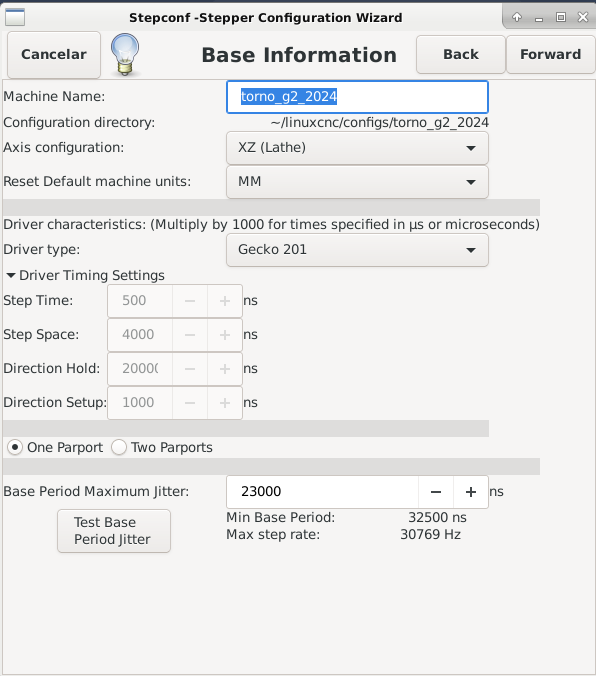
\includegraphics[width=0.95\textwidth]{images/prog/stepconf1.png}
    \end{center}
    \caption{Configuração inicial}\label{step1}
\end{figure}

Para que o LinuxCNC seja capaz de enviar sinais corretos para a caixa de controle a pinagem da porta paralela é definida em seguida. Essa pinagem foi disponibilizada para os alunos no moodle no inicio do curso e já foi apresentada anteriormente nesse relatório, porém, devido a peculiaridade da máquina girar seu eixo árvore no sentido anti-horário, a ferramenta foi colada do lado oposto ao usual, o que obrigou o grupo a inverter o sinal do pino que controla a direção do eixo X, de modo que avanços positivos comandados por código G realmente representassem uma aproximação da ferramenta em relação ao material usinado.

\begin{figure}[H]
    \begin{center}
        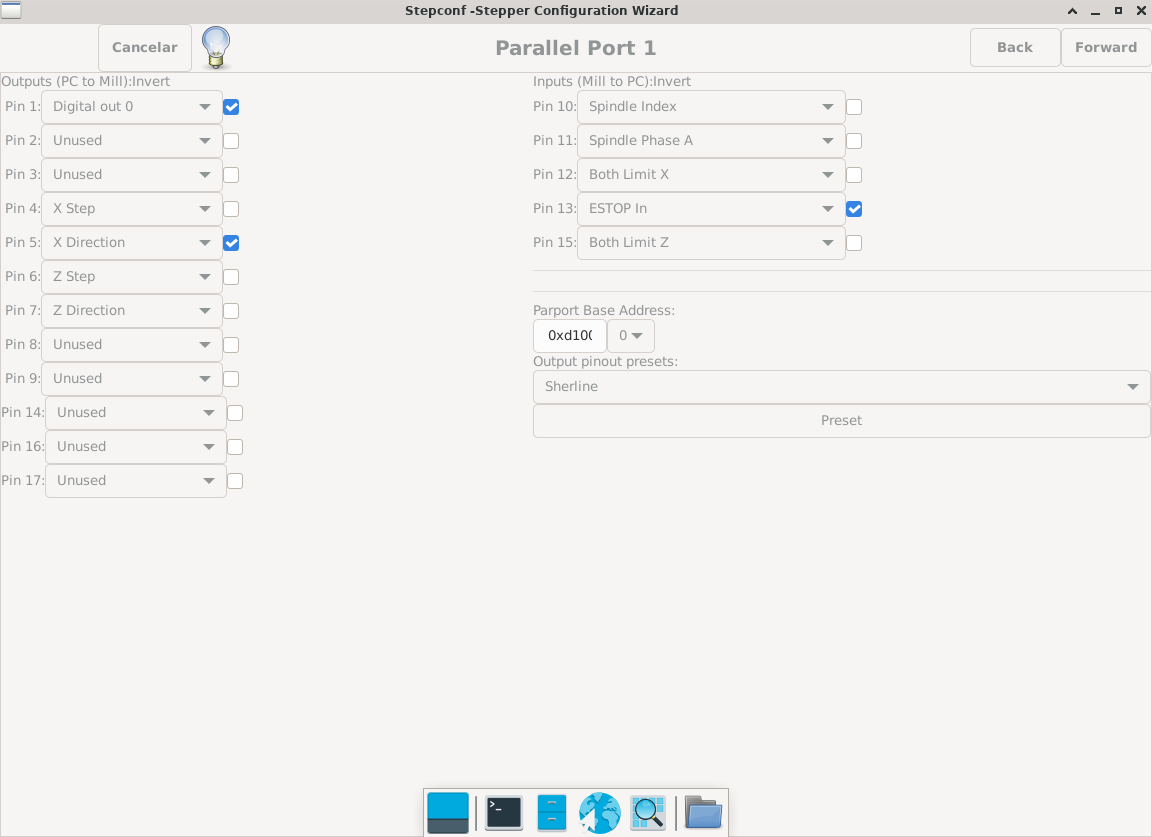
\includegraphics[width=0.95\textwidth]{images/prog/stepconf_config.png}
    \end{center}
    \caption{Configuração dos pinos da porta paralela}\label{pinagem}
\end{figure}

Os parâmetros de usinagem de cada eixo são definidos em seguida, sendo os mais relevantes as velocidades e acelerações máximas (25 mm/s e 750 mm/s, respectivamente) que foram definidos levando em consideração segurança de operação e integridade do equipamento (velocidades e acelerações muito grandes aumentam os riscos e as consequências de erros) e recomendações de técnicos que asseguraram ao grupo que essas configurações (que são o padrão) seriam mais que suficientes para as tarefas à serem executadas. Cabe ainda destacar que ambos os eixos receberam a mesma configuração, e que os seus limites estão definidos como valores muito grandes, uma vez que os verdadeiros limites foram definidos pelas chaves de fim de curso, não havendo assim necessidade de utilizar essa configuração para impor limites de deslocamento.

\begin{figure}[H]
    \begin{center}
        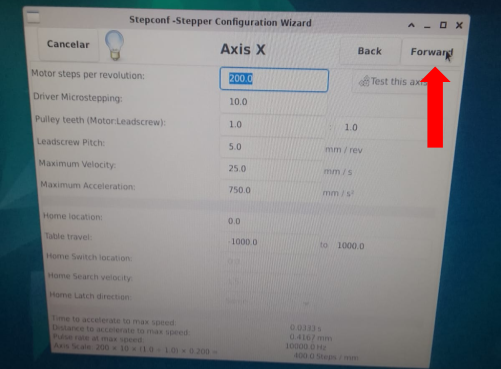
\includegraphics[width=0.95\textwidth]{images/Eletrica/Figura8.png} % lembrar de conseguir uma imagem melhor %
    \end{center}
    \caption{Configuração de um dos eixos}\label{eixos}
\end{figure}

\section{Configuração do controle manual}

Como requerimento de projeto foi pedido que o grupo mapeasse comandos do teclado que controlam os aspectos de controle manual da máquina no LinuxCNC para um Joystick, por meio de algum programa, de modo a facilitar o controle manual da máquina. Para realizar esse mapeamento, o grupo utilizou um fork do programa qjoypad, disponível na snapstore (problemas com a instalação serão tratados mais adiante na seção de desafios encontrados).
Foram mapeados para o Joystick os seguintes comandos:

\begin{itemize}
    \item Direita (d-pad direito, analógico) 
    \item Esquerda (d-pad esquerdo, analógico)
    \item Cima (d-pad acima, analógico)
    \item Baixo (d-pad abaixo, analógico)
    \item Aumentar velocidade (R1) 
    \item Diminuir velocidade (L1)
    \item Selecionar eixo X (L2)
    \item Selecionar eixo Z (R2)
    \item Homing do eixo selecionado (L3, R3, botão 3)
\end{itemize}

Abaixo, imagens das configurações feitas:

\begin{figure}[H]
    \begin{center}
        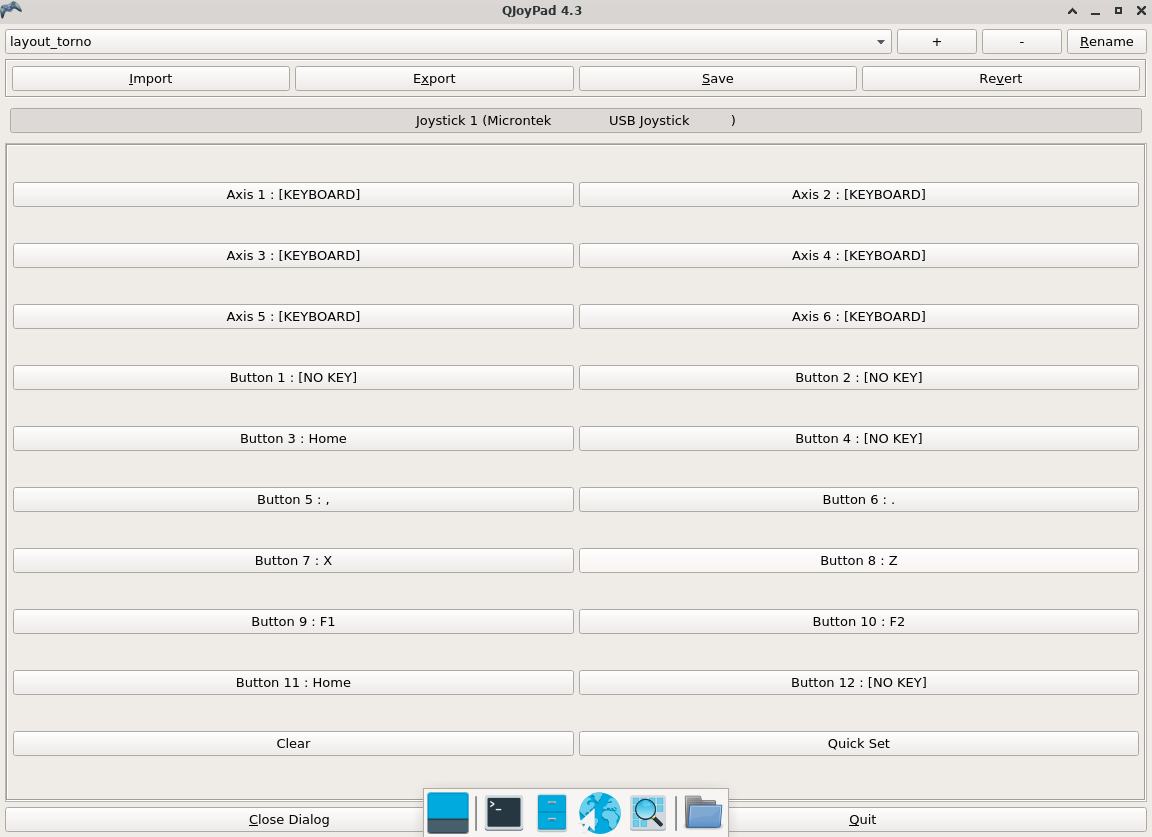
\includegraphics[width=0.95\textwidth]{images/prog/qjoypad_config.png}
    \end{center}
    \caption{Mapeamento feito no qjoypad}\label{qjoypad}
\end{figure}


\begin{figure}[H]
    \begin{center}
        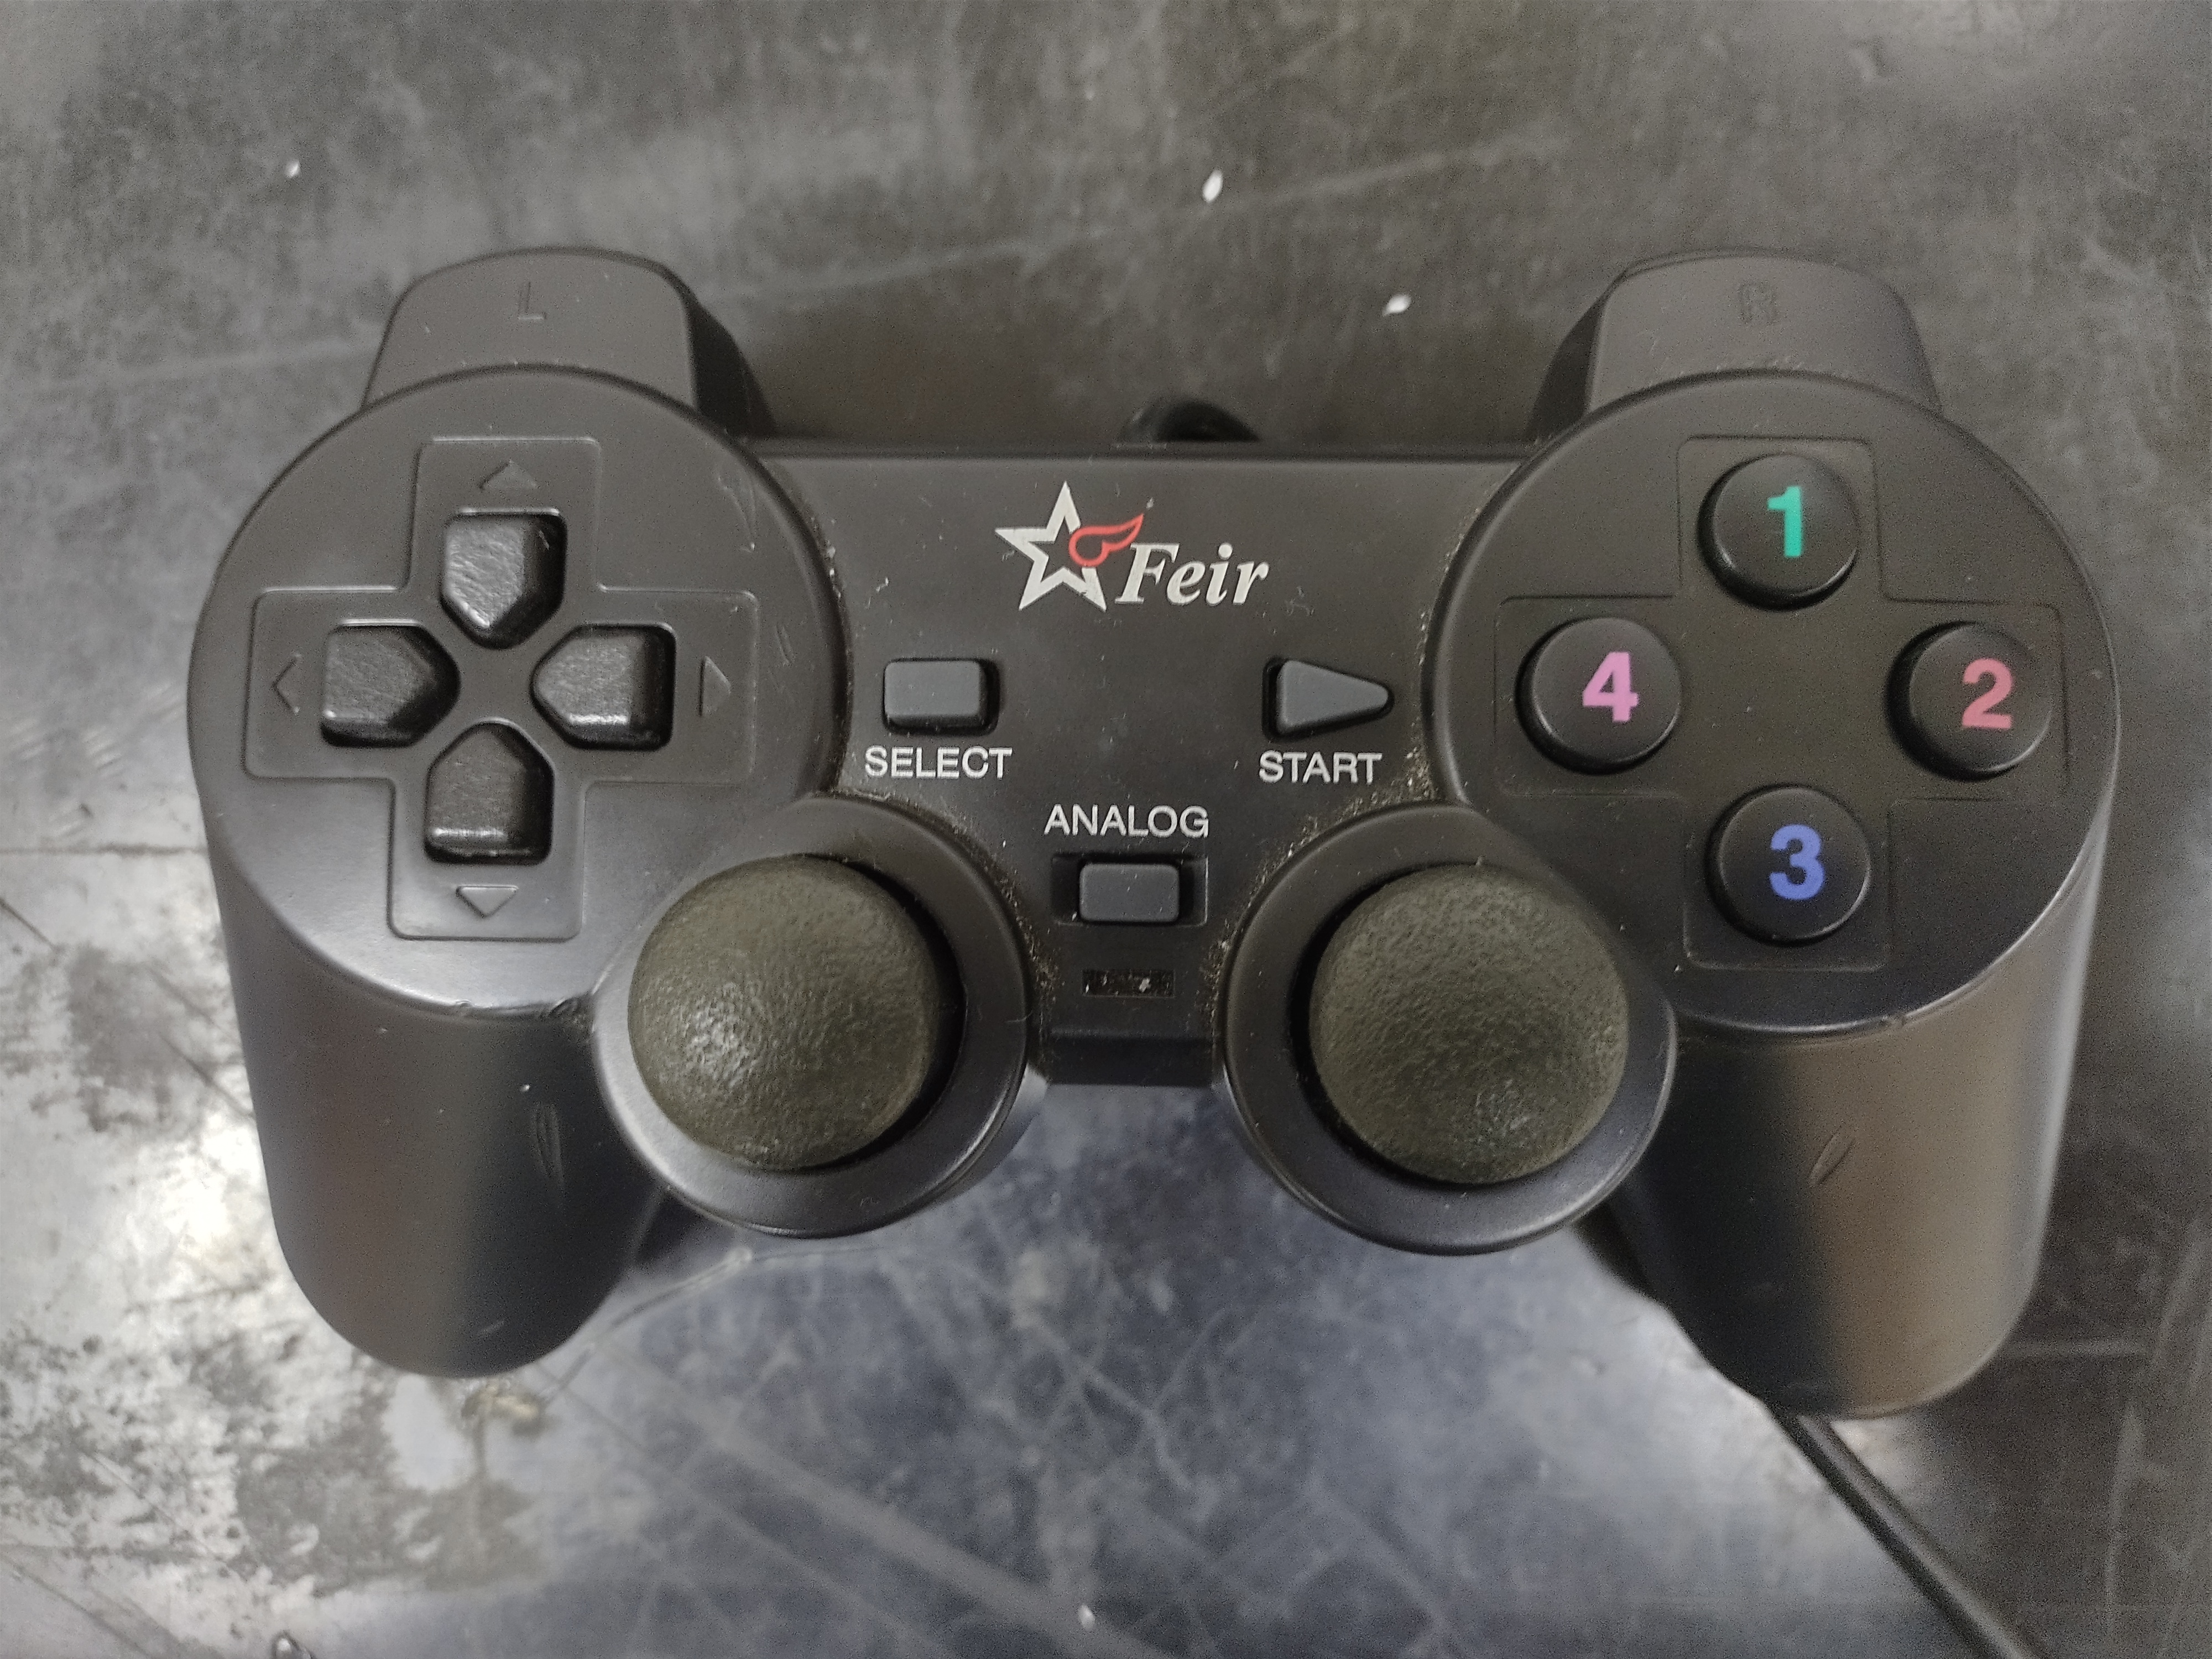
\includegraphics[width=0.95\textwidth]{images/prog/fotocontrole.png}
    \end{center}
    \caption{Comandos mapeados indicados no Joystick}\label{controle_joy}
\end{figure}

Cabe ressaltar que, para inicializar o qjoypad, e por consequência habilitar o controle manual no Joystick, é preciso executar o comando qjoypad no terminal. 

\section{Códigos G}
\subsection{Geração de códigos G}

A geração de códigos G se deu através da utilização da utilização do software Inventor CAM. A partir de um modelo também feito no Inventor, foram selecionados diversos parâmetros de usinagem de modo que uma simulação fidedigna de usinagem pudesse ser gerada. Os parâmetros mais relevantes estão listados a seguir: 

\begin{itemize}
    \item Tipo de ferramenta
    \item Velocidade de corte
    \item Velocidade de rotação
    \item Profundidade de corte máxima
    \item Fronteiras de corte
    \item Estratégia de corte
\end{itemize}

Como exemplo do que está descrito acima, seguem imagens da produção do CAM da peça final:

\begin{figure}[H]
    \begin{center}
        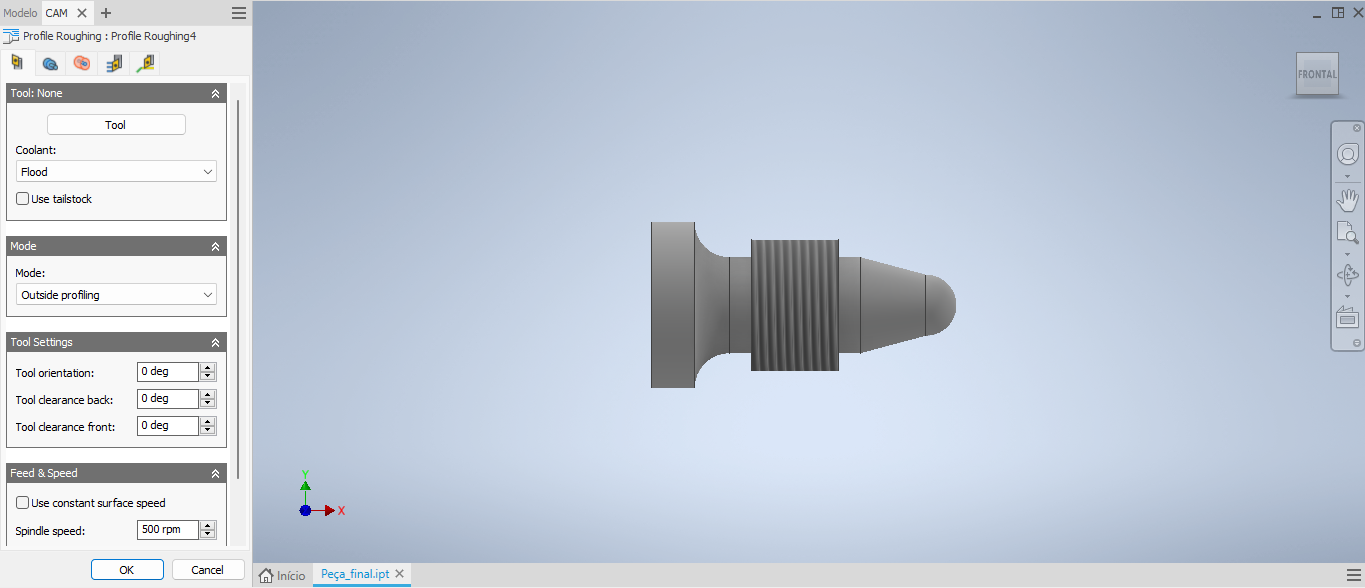
\includegraphics[width=0.95\textwidth]{images/prog/cam.png}
    \end{center}
    \caption{Interface onde são inseridas informações}\label{inicio_cam}
\end{figure}

\begin{figure}[H]
    \begin{center}
        \includegraphics[width=0.95\textwidth]{images/prog/cam_peça.png}
    \end{center}
    \caption{Caminho de desbaste gerado para a peça final}\label{cam_desbaste}
\end{figure}

\subsection{Tratamento do código G gerado}

Como os códigos gerados automaticamente não foram muito extensos, o grupo de programação lançou mão de revisões manuais para correção de eventuais erros. Erros comuns como o programa gerar códigos utilizando o código G32 (não suportado pelo LinuxCNC) ou utilizar coordenadas com nomenclatura U e W ao invés de X e Z podem ser facilmente resolvidos com o uso de uma função de encontrar e substituir, muito comum em editores de texto modernos. 

Para o ajuste de parâmetros de usinagem pontuais, como por exemplo velocidades, adição ou remoção de pausas para troca de ferramenta, e profundidades de corte, também se buscou usar de edições manuais no código, evitando a modificação de simulações no CAM ao máximo, apenas por uma questão de praticidade. Para tanto, o grupo instalou na máquina designada o editor Vscode, jundo de uma extensão que destaca sintaxe de código G.

\begin{figure}[H]
    \begin{center}
        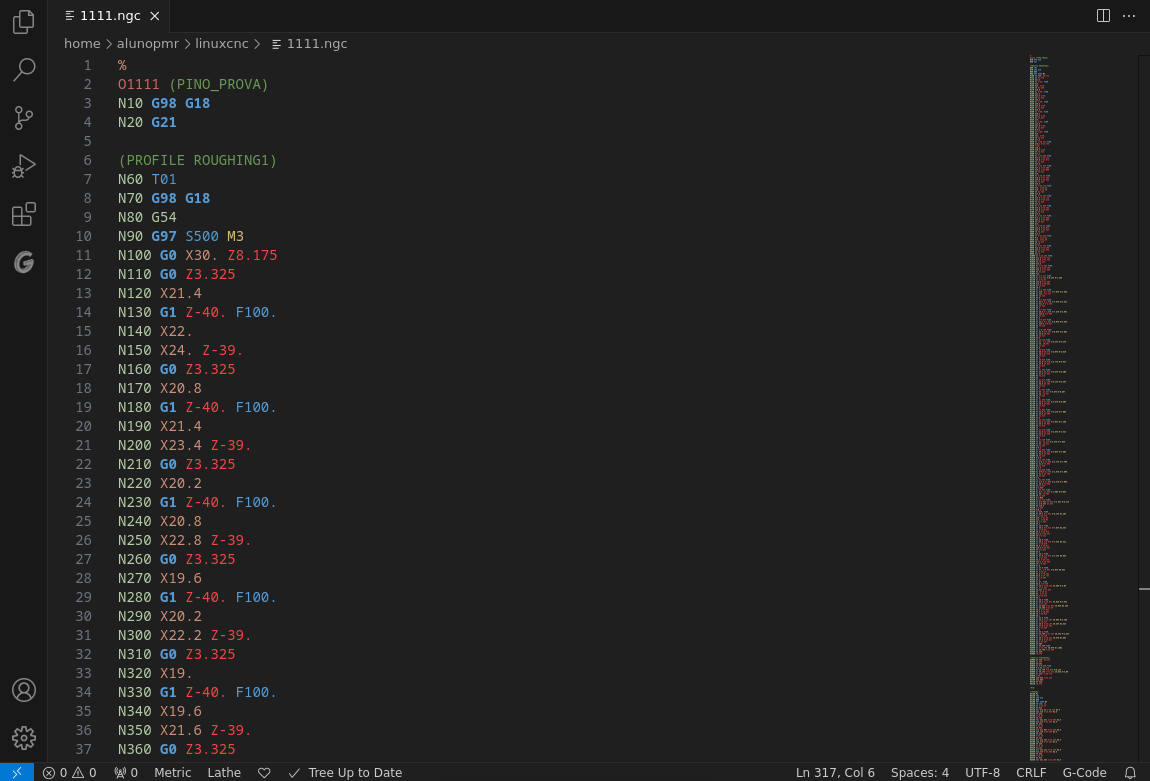
\includegraphics[width=0.95\textwidth]{images/prog/codigo_g.png}
    \end{center}
    \caption{Vscode com um código sendo editado}\label{code}
\end{figure}

Assim como o qjoypad, a instalação do Vscode foi feita através da instalação de um snap da snapstore.

\section{Procedimento de usinagem}

Idealmente, o grupo se reuniria para que os membros que soubessem operar a máquina repassassem esse conhecimento para os demais, o que de fato foi feito diversas vezes. Dito isso, o grupo de programação decidiu criar um manual de manuseio da máquina, de modo que todos pudessem estudar a máquina no horário que pudessem, evitando assim que a absência de membros do grupo por motivos adversos prejudicasse os demais. O procedimento descrito nos subtópicos a seguir é um resumo desse manual.

\subsection{Tratamento Inicial da Peça: Desbaste e Faceamento}

Antes de executar códigos G complexos, é essencial preparar a peça para a usinagem por meio de operações de desbaste e faceamento. Essas etapas garantem superfícies regulares e dimensões iniciais adequadas para a peça.

\subsection{Posicionamento Manual da Ferramenta}

Para ambas as operações, o operador deve posicionar a ferramenta manualmente:

\begin{itemize}
    \item Utilize o controle manual (Joystick ou teclado) para aproximar a ferramenta da peça.
    \item Ajuste a velocidade de avanço (Jog Speed) para um valor seguro, geralmente entre 20 e 50 mm/s.
    \item Posicione a ferramenta próximo à superfície da peça, garantindo uma pequena folga para evitar colisões.
\end{itemize}

\subsubsection{Desbaste}

O desbaste remove o excesso de material da superfície externa da peça, garantindo uniformidade ao diâmetro. Procedimentos principais:

\begin{itemize}
    \item Mova a ferramenta lateralmente ao longo do eixo Z, mantendo o eixo X fixo.
    \item Realize cortes sucessivos, reduzindo gradualmente o diâmetro até atingir o valor desejado.
    \item Monitore visualmente o processo e ajuste a velocidade de avanço conforme necessário.
\end{itemize}

\subsubsection{Faceamento}

O faceamento nivela a face da peça, removendo irregularidades. Etapas:

\begin{itemize}
    \item Posicione a ferramenta próxima à extremidade frontal da peça.
    \item Mova a ferramenta ao longo do eixo X, com o eixo Z fixo.
    \item Realize cortes suaves e uniformes até que toda a face da peça esteja nivelada.
\end{itemize}

Ambas as operações devem ser realizadas com cuidado para evitar colisões e assegurar que a peça esteja firme na placa de fixação.

\subsection{Configuração Inicial do Ambiente de Programação}

Antes de iniciar a programação efetiva do torno, é preciso preparar o ambiente de execução do LinuxCNC. Alguns pontos-chave:

\begin{itemize}
    \item \textbf{Ligação dos dispositivos:} É recomendável que a caixa de controle da máquina esteja ligada e o Joystick conectado antes da inicialização do computador. Isso previne problemas de detecção de periféricos pelo LinuxCNC.
    \item \textbf{Login e Sistema:} Após ligar o computador (com caixa de controle já energizada), efetua-se o login no sistema operacional. 
    \item \textbf{Execução do LinuxCNC:} Com o LinuxCNC aberto, deve-se selecionar a configuração apropriada do torno. Uma vez carregada a interface principal, o usuário pode então dar início à programação e à interação com o ambiente de usinagem.
\end{itemize}

\subsection{Referenciamento (Homing) e Modos de Coordenadas}

Um passo fundamental na etapa de programação é o homing dos eixos (X e Z). Esse processo estabelece a posição de referência absoluta da máquina, conhecida como zero máquina, imprescindível para qualquer subsequente programa em código G. 

Após realizar o homing, o usuário pode definir planos de corte (por exemplo, G54) e zeros de peça, garantindo que o código G seja interpretado corretamente em relação à posição física da ferramenta e do tarugo a ser usinado.

\subsubsection{Definição do Zero Peça}

Definir o zero peça envolve posicionar a ferramenta em contato com o material e, através de recursos do LinuxCNC (como o apalpador), informar ao controlador o deslocamento necessário. Para o eixo Z, posiciona-se a ferramenta na face do tarugo; já para o eixo X, é necessário conhecer o diâmetro do tarugo. Essa informação garante que o código G seja interpretado corretamente, especialmente ao trabalhar em modo de diâmetro (G7).

O correto ajuste do zero peça é determinante para assegurar que o caminho programado no código G resulte em movimentos seguros e precisos, evitando colisões e garantindo o correto posicionamento da ferramenta em relação à geometria desejada.

\subsection{Carregando e Executando Código G}

A programação do torno CNC via LinuxCNC baseia-se na leitura e execução de arquivos com extensão \textit{.ngc}, contendo instruções G-code. Após ajustar o zero peça e conferir se o modo de diâmetro (G7) está ativado quando necessário, o usuário pode abrir o arquivo desejado:

\begin{itemize}
    \item \textbf{Seleção do Programa:} Através da interface gráfica do LinuxCNC, o usuário seleciona o arquivo \textit{.ngc} a ser executado.
    \item \textbf{Pré-visualização:} Antes da execução, o preview mostra o caminho da ferramenta, permitindo checar visualmente se o trajeto faz sentido.
    \item \textbf{Execução:} Ao dar início à execução, o LinuxCNC seguirá as instruções do código G, respeitando parâmetros de avanço, velocidade e comandos de mudança de ferramenta.
\end{itemize}

Durante este processo, é possível ajustar fatores como a velocidade máxima de execução, garantindo maior segurança caso haja incerteza sobre o comportamento do programa.

\section{Desafios encontrados}

Além dos problemas recorrentes e simples de serem solucionados, como por exemplo o ajuste de códigos G (ou até mesmo eventuais modificações em um CAM) além de afiações e ajustes de ferramenta para garantir que o torno produzisse resultados adequados, o grupo de programação deve de superar alguns desafios que merecem destaque. Nos subtópicos a seguir estes desafios serão listados e discutidos.

\subsection{Modo de diâmetro (G07)}

Sem dúvidas esse foi o erro que custou mais tempo do grupo de programação (cerca de uma semana para a solução). Esse erro foi observado pela primeira vez ao se tentar produzir uma peça com um raio esférico na sua ponta, o que gerou uma mensagem de erro que indicava o que aparentemente eram dois raios distintos e conflitantes no código.

\begin{figure}[H]
    \begin{center}
        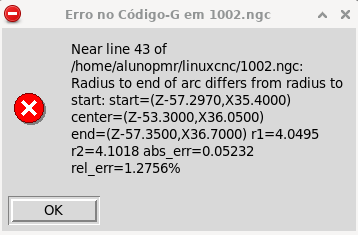
\includegraphics[width=0.95\textwidth]{images/prog/erro_g7.png}
    \end{center}
    \caption{Erro apresentado quando G07 não está ativo}\label{g07}
\end{figure}

O fato de que ninguém para o qual nós apresentamos esse erro pôde identificar erros no código G indicou para o grupo que havia um erro desconhecido ocorrendo no interpretador do LinuxCNC. Como nada do que foi tentado funcionou, a medida de trocar o computador e copiar a configuração de ambiente de outro grupo que teve seu sistema operacional atualizado foi tomada, porém isso não solucionou o problema. 

No fim, o grupo descobriu, ao observar a indicação da posição do eixo X na interface gráfica, que o comportamento padrão do LinuxCNC presente na máquina era de ter o modo de coordenadas em raio ativado, o que é incomum para códigos de usinagem CNC. Assim, a única solução encontrada foi a ativação do código G07 a partir do MDI antes de carregar qualquer código G. 

Além do tempo necessário para finalmente descobrir a causa real do problema, a maior parte do tempo gasto devido a esse erro veio do fato de o grupo ter de configurar o ambiente de execução novamente devido a troca de computador. Além disso, essa troca foi a causa do próximo problema que será discutido. 

\subsection{Instalação do qjoypad}

Inicialmente o programa qjoypad já estava instalado na máquina que o grupo recebeu, de modo que o trabalho de configurar o controle manual se resumiu à apenas mapear os comandos no aplicativo. No entanto, devido a troca de computador e atualização de sistema operacional, o programa teve de ser instalado novamente. 

O processo de instalação do aplicativo original, disponível na Source Forge, é simplesmente a sua compilação a partir dos arquivos fonte. Porém isso não foi possível, pois o sistema operacional recentemente instalado não possuía uma ferramenta de compilação chamada de \textbf{qmake}, a qual tinha um processo de instalação que precisaria de internet para ser viável. 

Já com acesso a internet, por meio de roteamento à partir de telefones móveis, foi constado que a instalação de qualquer pacote seria muito dificultada pois o sistema não tinha nem uma lista dos repositórios remotos padrões do Debian, provavelmente devido ao tipo de instalação feita (totalmente offline). Finalmente ao achar o arquivo de configurações de fontes remotas do Debian, foram adicionadas as seguintes fontes:

\begin{figure}[H]
    \begin{center}
        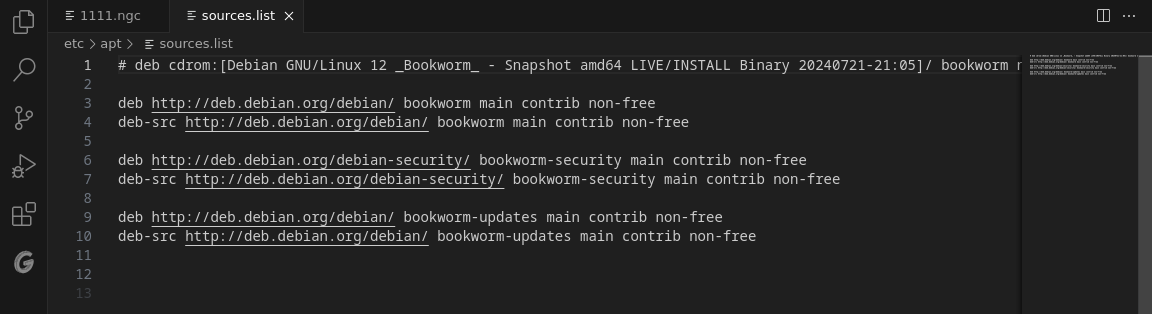
\includegraphics[width=0.95\textwidth]{images/prog/fontes.png}
    \end{center}
    \caption{Repositórios remotos adicionados}\label{fontes}
\end{figure}

Com essas fontes instaladas, foi possível instalar a snapstore e, a partir dela, um snap de um fork mais novo do qjoypad, com as mesmas funcionalidades do original.

\subsection{Reconhecimento de periféricos}

Esse problema se manifesta pelo fato do LinuxCNC instalado na primeira máquina que o grupo recebeu não procurar por periféricos após a inicialização, o que significa que qualquer dispositivo que o grupo quisesse conectar em alguma porta USB, como por exemplo o Joystick ou um pendrive, deveria ser conectado antes da inicialização. Esse problema simplesmente entrou para o procedimento de usinagem como um aviso de conectar tudo antes de ligar o computador. 

Após a troca de computador, no entanto, o LinuxCNC se tornou capaz de reconhecer periféricos conectados após a inicialização, então o problema foi definitivamente resolvido após a atualização.
